\subsection{Implementierung}

\subsubsection{Inbetriebnahme der Hardware}
Der erste Teil der Implementierung sah die Bereitstellung von Treibern für die Hardware des Volksbots vor. Die Initialisierung und Ansteuerung der an den EPOS2-Controllern angeschlossenen Peripherie erfolgte unter der Verwendung der EPOS2 Bibliothek. Diese Bibliothek verfügt über alle benötigten Funktionen zum Ansteuern und Auslesen der Motoren und Lichtschranken, welche mit den EPOS-Controllern verbunden sind. Die Funktionen wurden in einem ROS-Package namens „epos2-control“ zusammengeführt.
Die Verwendung der Laserscanner wurde durch die Implementierung und Parametrisierung von im ROS vorhandenen Treibern gewährleistet. Dem an der Front des Roboters angebrachten SICK LMS100 Laserscanner, wurde dafür unter Windows eine feste IP-Adresse zugeordnet. Mit Hilfe dieser bekannten Adresse, konnte auch unter Ubuntu die Verbindung über Ethernet mit dem Laserscanner durch das Package „LMS1xx“  hergestellt werden.

\begin{figure}[h!]
 \centering
		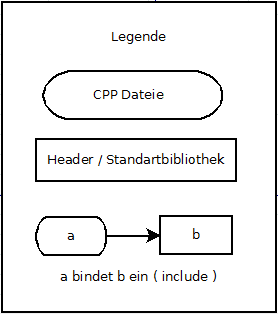
\includegraphics[width=0.4\textwidth]{Legende.png}
	\caption{Legende zu Abb. 46 und 47}
	\label{fig:Legende}
\end{figure}

\begin{figure}[h!]
 \centering
		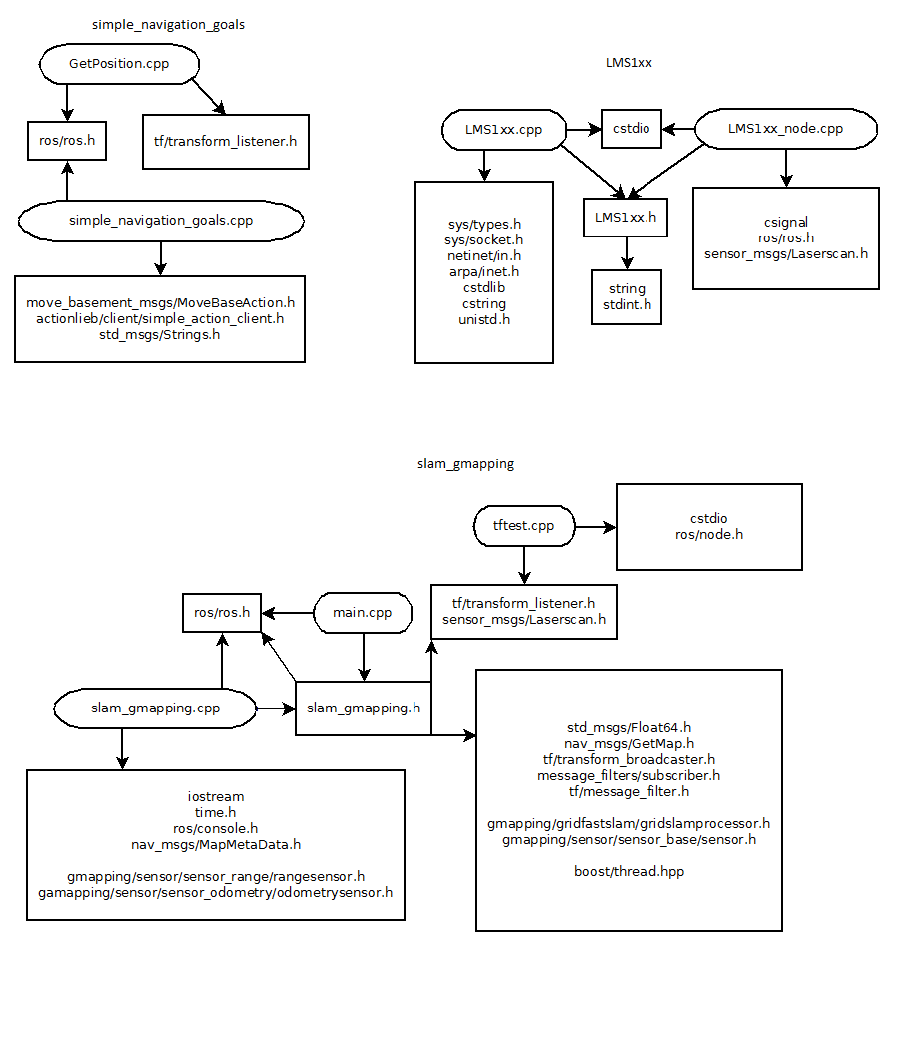
\includegraphics[width=1\textwidth]{funktionen.png}
	\caption{eingebundene Funktionen in ROS}
	\label{fig:funktionen}
\end{figure}

\begin{figure}[h!]
 \centering
		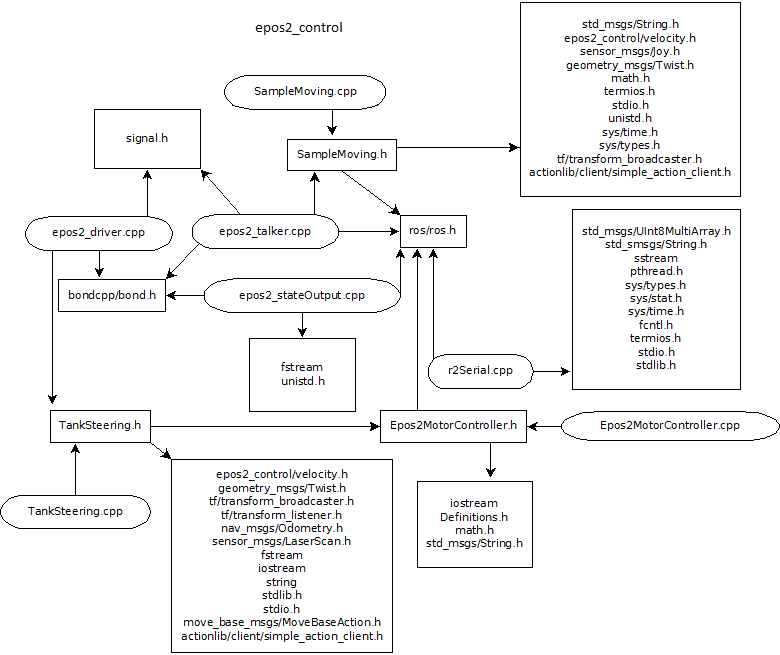
\includegraphics[width=1\textwidth]{epos2_control.png}
	\caption{Hauptsteuerung des Systems ( Epos2 Control )}
	\label{fig:epos2_control}
\end{figure}

\subsubsection{Implementierung der Navigation}
Nach erfolgreicher Inbetriebnahme der Hardware des Volksbots wurde die Odometrieberechnung anhand der zurückgelegten Strecke der Räder implementiert. Die Berechnung der zurückgelegten Wegstrecke und der Drehung des Roboters erfolgt über folgende Formeln: … FORMELN EINFÜGEN (Referenz: Der und Pantzer Odometrie oder Mobile Roboter Buch)
Die Daten der Odometrie werden zur Lokalisierung des Roboters innerhalb einer mit dem SICK LMS100 Laserscanners erstellten Umgebungskarte verwendet. Die Implementierung erfolgte ebenso wie bei der Entwicklung der Treiber im „epos2-control“-Package. Bei der Erstellung der Umgebungskarte wurde auf das „Gmapping“-Package von ROS zurückgegriffen. Der darin enthaltene Algorithmus nutzt die Daten des Laserscanners, um während der Fahrt des Roboters aus seiner erfassten Umgebung eine Karte zu erstellen. Zur Visualisierung der Karte und der Daten des Laserscans wurde „Rviz“, ein Visualisierungstool innerhalb der ROS-Umgebung verwendet. Mit Hilfe von Rviz ist es neben der Visualisierung unter anderem möglich die initiale Position des Roboters, sowie Navigationsziele innerhalb der Karte festzulegen. (Screenshot Rviz) Mit dem Ziel den auftretenden Abweichungen der Odometrieberechnung entgegenzuwirken, wurde das „adaptive Monte Carlo Localisation“-Package (AMCL) implementiert. Vereinfacht formuliert, nutzt dieses Verfahren die Daten des Laserscans und der Karte, um mit Hilfe der Merkmale des aktuellen Scans und der zugrundeliegenden Daten der Kartenrepräsentation eine Schätzung der Position des Roboters auszuführen. (Referenz: AMCL Diplomarbeit Manuela B)
Eine funktionsfähige Selbstlokalisation ist die Grundlage für eine erfolgreiche autonome Navigation in der Umgebung des Roboters. Das ROS-Framework stellt mit dem „move-base“-Package die nötigen Funktionen für die Navigation bereit. Das Package hat den Dijkstra-Suchalgorithmus zur Wegplanung implementiert und nutzt zwei parametrisierbare Costmaps, um Eigenschaften wie z.B. den Mindestabstand zu Hindernissen oder das Verhalten bei Planungsfehlern festzulegen. Nach der Planung der Navigation werden die passenden Steuerbefehle generiert. Falls der Volksbot in eine unvorhergesehene Situation gerät und seine geplante Route nicht mehr gültig ist, kommen Recovery-Funktionen des Packages zum Einsatz. Dabei wird eine Rotation um die eigene Achse des Roboters durchgeführt, um einen geeigneten Ausweg zu finden. 

\subsubsection{Implementierung der Paketübergabe}
Damit der Austausch der Pakete mit den Komponenten des Materialflusses erfolgen kann, musste die Kommunikation über die MICAz-Module und Automatismen zur Anpassung der Hub-Position an die Höhe der jeweiligen Rampe implementiert werden. Nachdem ein Auftrag vom Materialfluss empfangen wurde, wird die Annahme des Auftrags dem Materialfluss bestätigt und der Auftrag  in ein passendes Navigationsziel auf der Umgebungskarte umgesetzt.  Für den Prozess des Entschlüsselns von den Nachrichten des Materialflusses wurde ein ROS-Package namens „Simple-Navigation-Goals“ implementiert. Neben der Umsetzung von Navigationszielen sendet dieses Package ROS-interne Nachrichten, welche Informationen über die gewünschte Position des Hubs und das Erreichen der Zielposition enthalten.
Sobald die Zielposition erreicht wurde, beginnt die Hubsteuerung mit der Anpassung der Hubposition an die geforderte Höhe. Anschließend folgt eine Benachrichtigung an den Materialfluss und das Förderband wird in Gang gebracht. Die Auswertung der Lichtschranken bewirkt den Haltevorgang des Förderbands und das nächste Navigationsziel wird festgelegt.

\subsubsection{Struktur der einzelnen Funktionalitäten}



